%! Author = fabian
%! Date = 21.11.21

% Preamble
\documentclass[a4paper]{article} % Uses article class in A4 format

%----------------------------------------------------------------------------------------
%	FORMATTING
%----------------------------------------------------------------------------------------

\addtolength{\hoffset}{-2.25cm}
\addtolength{\textwidth}{4.5cm}
\addtolength{\voffset}{-3.25cm}
\addtolength{\textheight}{5cm}
\setlength{\parskip}{0pt}
\setlength{\parindent}{0in}


%----------------------------------------------------------------------------------------
%	PACKAGES AND OTHER DOCUMENT CONFIGURATIONS
%----------------------------------------------------------------------------------------

\usepackage[utf8]{inputenc} % Use UTF-8 encoding
%\usepackage{microtype} % Slightly tweak font spacing for aesthetics

\usepackage[english]{babel} % Language hyphenation and typographical rules

\usepackage{amsthm, amsmath, amssymb, bm} % Mathematical typesetting
\usepackage{float} % Improved interface for floating objects
%\usepackage[final, colorlinks = true,
%linkcolor = black,
%citecolor = black]{hyperref} % For hyperlinks in the PDF
\usepackage{graphicx, multicol} % Enhanced support for graphics
\usepackage{subcaption}
\usepackage{xcolor} % Driver-independent color extensions
%\usepackage{marvosym, wasysym} % More symbols
%\usepackage{rotating} % Rotation tools
%\usepackage{censor} % Facilities for controlling restricted text!
%\usepackage{booktabs} % Enhances quality of tables
%\usepackage{censor} % Facilities for controlling restricted text!
%\usepackage{booktabs} % Enhances quality of tables
\usepackage{listings}
\usepackage{enumitem}
\usepackage{caption}

%\usepackage{csquotes} % Context sensitive quotation facilities
\usepackage[yyyymmdd]{datetime} % Uses YEAR-MONTH-DAY format for dates
\renewcommand{\dateseparator}{-} % Sets dateseparator to '-'

\usepackage{fancyhdr}
\usepackage{amsmath}
\usepackage{bm}
\usepackage{amsfonts} % Headers and footers
\pagestyle{fancy} % All pages have headers and footers
\fancyhead{}\renewcommand{\headrulewidth}{0pt} % Blank out the default header
\fancyfoot[L]{} % Custom footer text
\fancyfoot[C]{} % Custom footer text
\fancyfoot[R]{\thepage} % Custom footer text

%\newcommand{\note}[1]{\marginpar{\scriptsize \textcolor{red}{#1}}} % Enables comments in red on margin
\DeclareMathOperator*{\argmax}{argmax}
\DeclareMathOperator*{\argmin}{argmin}
%----------------------------------------------------------------------------------------

% Document
\begin{document}
%----------------------------------------------------------------------------------------

%	TITLE SECTION
    \title{Title} % Article title
    \fancyhead[C]{}
    \hrule \medskip % Upper rule
    \begin{minipage}{0.295\textwidth} % Left side of title section
        \raggedright
        TTK4255\\ % Your lecture or course
        \footnotesize % Authors text size
        \hfill\\
        Fabian Höldin % Your name, your matriculation number
    \end{minipage}
    \begin{minipage}{0.4\textwidth} % Center of title section
        \centering
        \large % Title text size
        Robotic Vision \\ % Assignment title and number
        \normalsize % Subtitle text size
        Midterm project: Model-based pose estimation\\ % Assignment subtitle
    \end{minipage}
    \begin{minipage}{0.295\textwidth} % Right side of title section
        \raggedleft
        \today\\ % Date
        \footnotesize % Email text size
        \hfill\\
        % Your email
    \end{minipage}
    \medskip\hrule % Lower rule
%----------------------------------------------------------------------------------------
%	ARTICLE CONTENTS
%----------------------------------------------------------------------------------------

\section{Estimate the helicopter angles}
    \subsection*{Task 1.1}
    \subsection*{Task 1.2}
    \subsection*{Task 1.3}
    Optimal angles (residuals) on image 0:
    \begin{center}
        \begin{tabular}{ccccccc}
            5.24245604 & 4.80020124 & 1.19885845 & -4.99317996 & -4.47286417 & 0 & 0.04965743 \\
            -8.87519959 & -5.02385631 & -6.06002405 & -2.97156827 & 0.43079638 & 0 & -6.26710301
        \end{tabular}
    \end{center}
    \begin{figure*}[h]
        \centering
        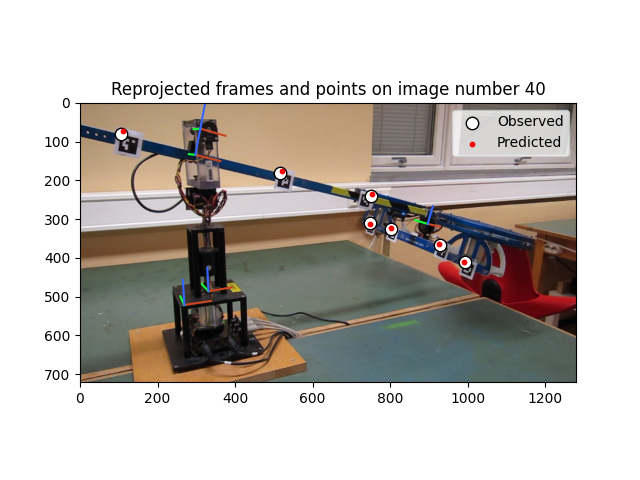
\includegraphics[width= 0.7 \linewidth]{../python/out_part1a_10steps}
    \end{figure*}
    Reprojection errors at solution:\\
    Marker 1: 10.60 px\\
    Marker 2:  7.26 px\\
    Marker 3:  5.06 px\\
    Marker 4:  2.70 px\\
    Marker 5:  1.85 px\\
    Marker 6:  3.57 px\\
    Marker 7:  1.90 px\\
    Average:   4.71 px\\
    Median:    3.57 px

    \subsection*{Task 1.4}
    \begin{center}
        \begin{tabular}{cccc}
            \hline
            $\bm{p_0}$ & steps & Avg.Err. & Med.Err \\
            \hline \hline
            $ \bigl[ \begin{smallmatrix}
                         0.0 & 0.0 & 0.0
            \end{smallmatrix} \bigr] ^T$ &
            3 & 4.71 px & 3.38 px\\
            $ \bigl[ \begin{smallmatrix}
                         0.5 & 0.5 & 0.5
            \end{smallmatrix} \bigr] ^T$ &
            3 & 4.71 px & 3.61 px \\
            $ \bigl[ \begin{smallmatrix}
                         1.0 & 1.0 & 1.0
            \end{smallmatrix} \bigr] ^T$ &
            4 & 4.71 px & 3.80 px\\
        \end{tabular}
    \end{center}
    As can be seen in the above table, the initial value $\bm{p_0}$ does not change the amount of steps nor the reprojection error significantly.

    \subsection*{Task 1.5}
    We get this warning because we are trying to solve an under-determined system of linear equations what results in having infinite many solutions.
    The "numpy.linalg.solve()" function cannot handle this.

    \subsection*{Task 1.6}
    For simply extending the dimensions $\bm{p} \in \mathbb{R}^4$ we will get a Jacobian $ \bm{J} \in \mathbb{R}^{n \times 4}$ and an approximate Hessian $\bm{J}^T \bm{J} \in \mathbb{R}^{4 \times 4} $.
    The modification of the helicopter model might result in not having unique configurations for one specific model state, e.g. $\phi$ and $\psi$ are nearly indistinguishable for straight upwards pointing helicopter.

    \subsection*{Task 1.7}
    \begin{enumerate}[label=(\alph*)]
        \item The maximum error is 19.4877 pixels.
        \item This maximum error occurs in image 104.
        The minimum error occurs in image 152.
        \item Parameter : \\
        - Yaw: max = 0.7999 , image: 187 \\
        - Pitch: max = 0.2431, image: 327 \\
        - Roll: max = 0.0748, image: 350 \\
        The minimum errors are 0 at image 0 because of the offset synchronization we use.
    \end{enumerate}

    \subsection*{Task 1.8}
    \begin{enumerate}[label=(\alph*)]
        \item Because of the way the residue function has been implemented, with the weights for valid entries, the residue of unobserved markers are set to zero.
            Followingly, the corresponding index of the jacobian matrix $J$ will be zero too - leading to a potentially singular matrix, which prevents solving for a unique solution.
            The Levenberg-Marquardt method has circumvented this problem by fixing the step length to 1 and adding a term $\mu*I$ to the normal equation.
            This guarantees that the equation remains solvable and that the estimation algorithm can move past the points with insufficient observational data.
        \item The added term $\mu I$ adds $\mu 1$ to the diagonal elements of $J^TJ$, with \mu having a variable magnitude.
            The Levenberg-Marquardt method is set up in such a way that the $\mu$ term decreases when approaching the minimum, and increases otherwise.
            This means that the $J^TJ$ term will dominate when close to the minimum, leveraging the benefits of Newton-Gauss, while having the '+1' term dominate further from the minimum - where Newton-Gauss struggles.
            The downside of this method, is the fixed step length of 1.
            While Levenberg-Marquardt is robust in ensuring that each step of the optimization remains solvable, it suffers from a sort of 'maximum accuracy' - with no guarantees beyond 'minimum + 1'.
            This must be taken into account when determining the stopping criterion.
    \end{enumerate}


\end{document}
